% No clue what this does
\documentclass{article}

% allow useage of graphics 
\usepackage[pdftex]{graphicx}
\usepackage{wrapfig}
%\usepackage[final]{graphicx}
%\usepackage[dvipdfmx]{graphicx} 
%\usepackage{bmpsize}

% Allow the usage of utf8 characters
\usepackage[utf8]{inputenc}

% The maths package
\usepackage{amsmath}
% For double line element like R, C or Z
\usepackage{amsfonts}
% For double line element like 1, 2, ..
\usepackage{dsfont}
% For is defined as symbol (coloneqq)
\usepackage{mathtools}
% for Proof paragraphs
\usepackage{amsthm}

%subitem bulletpoints
\usepackage{outlines}

% bibtex style
\usepackage{apacite}

% a packages just used for the tabulator for the pascals triangle
\usepackage{array}

% package to alighn images
%\usepackage[export]{adjustbox}
\usepackage{float}
\usepackage{subcaption}

% use the tikz package, no clue why I need the positioning thing
\usepackage{tikz}
\usetikzlibrary{positioning}

% as it sais. Start the section counter from zero
% instead of starting it at one
\setcounter{section}{-1}

\theoremstyle{definition}
\newtheorem{theorem}{Theorem}[section]
\newtheorem{corollary}[theorem]{Corollary}
\newtheorem{lemma}[theorem]{Lemma}
\newtheorem{definition}[theorem]{Definition}
\newtheorem{proposition}[theorem]{Proposition}
\newtheorem{comment}[theorem]{Comment}
\newtheorem{remark}[theorem]{Remark}

% create a command to easyly add figure titles
\newcommand*{\figuretitle}[1]{%
    {\centering%   <--------  will only affect the title because of the grouping (by the
    \textbf{#1}%              braces before \centering and behind \medskip). If you remove
    \par\medskip}%            these braces the whole body of a {figure} env will be centered.
}

\title{Tropical Geometry of Deep Neural Networks}
\author{David Leatham}
\date{\today}

% Start the document
\begin{document}


%\maketitle
\begin{titlepage}
	\begin{center}
		\vspace*{2.5cm}
		\begin{LARGE}
		Bachelor Thesis
		\end{LARGE}
		
		\vspace{0.3cm}
		\LARGE
		\textbf{Tropical Geometry of \\ Deep Neural Networks}
		
		\vspace{1cm}
		
		\large
		David Leatham \\
		\vspace{0.2cm}
		\large
		\today
		
	\end{center}
	
\end{titlepage}

\newpage
  
\tableofcontents

\newpage


% Create a new 0th level heading named Introduction
\section{Introduction} 
\leavevmode
\\
Tropical geometry is historically a modern branch of mathematics subject to a rise in research observed through out the past 30 years. Neural networks have found application in many disciplines and have been used to algorithmically manage abstract tasks like self driving cars, face and text recognition or automatically processing hand written checks at banks. Neural networks impact our lives on a daily basis. \\
In this thesis we describe a new representation of neural networks through tropical geometry, following recent research of the past two years, making this a very contemporary topic. \\

Warren McCulloch and Walter Pitts opened the subject of neural networks in 1943 by creating a computational model for neural networks. In the following years one of the next big steps towards today's state of the art neural networks, is in the early 60's with research into the underlying concepts of backpropagation. Backpropagation is an algorithm describing a key concept of training neural networks. Starting $2010$ to this day neural networks are experiencing a massive boost in popularity, which is due to hardware improvements like GPU's, making backpropagation feasible with large amounts of data and the improvement of underlying understanding as of works by Andrew Yan-Tak Ng and Jeff Dean who in 2012 created a network that learned to recognize higher-level concepts, such as cats, only from watching unlabeled images \cite{DBLP:journals/corr/abs-1112-6209}. Nowadays neural networks help solve challenging problems in computer science and software engineering and in particular are key to application areas such as system identification and control, pattern and sequence recognition, social network filtering and e-mail spam filtering. \\
Tropical geometry on the other hand is a field of interest in mathematics, whose underlying analytical ideas have been around some years before $1990$, but only since then have there been basic efforts to consolidate the basic definitions as research increased. Tropical geometry is the study of polynomials under tropical multiplication and addition, where tropical multiplication is usual addition and tropical addition of two elements returns the minimal element. One spectrum of use cases is in computer science and this work is a very good example for that, as in this thesis we describe a fundamental mathematical connection between tropical geometry and deep neural networks. \\

Concerning the structure of the thesis we start by introducing the reader to the necessary theories of tropical geometry in chapter \ref{sec:trop_algebra} and the theory of neural networks in chapter \ref{sec:neural_networks}, but also extend the exploration of the topics beyond the scope needed for the fundamental Theorems in this thesis to give a more rounded introduction to the topics themselves when appropriate. Chapter \ref{sec:trop_netw} uses the knowledge of these two chapters to demonstrate a fundamental link between neural networks and the difference between two tropical polynomials, called tropical rational functions, which is the core insight of the thesis.
Then, to put this knowledge to use, we formulate statements about decision boundaries of neural networks in chapter 5 with tropical geometry, or more concrete, the link between neural networks and tropical rational functions. This needs fundamental knowledge of tropical hypersurfaces which leads us to to chapter \ref{sec:tropical_hypersurfaces} in which these are introduced. \\

This thesis follows the underlying paper \cite{maclagan2015introduction} very closely, in that all main statements may be reordered and rewritten, but come directly out of \cite{maclagan2015introduction} and are cited accordingly.

\newpage

\section{Tropical Algebra}
\label{sec:trop_algebra}
We begin by introducing the theory of tropical algebra. Every other chapter will build upon chapter \ref{sec:trop_algebra} without exception. The main goal is to build an intuition and formal understanding of tropical / tropical rational functions and maps. \\

Our basic object of study is the object $( \mathbb{R} \cup \{- \infty \} , \oplus , \odot )$. As a set this corresponds to the real numbers $ \mathbb{R} $, together with an extra element $- \infty $ which represents minus infinity. In this (semiring) the tropical sum of real numbers is their maximum and the tropical product of real numbers is their usual sum 
$$ x \oplus y := \max(x,\ y) \quad \text{and} \quad x \odot y := x+y.$$
In Tropical Geometry often infinity instead of minus infinity and $\min$ instead of $\max$ are used. This does not change any of the underlying theories of tropical algebra as the two semirings are tropically Isomorph. Meaning 
\begin{align*}
( \mathbb{R} \cup \{- \infty \} , \oplus := \max, \odot ) &\to ( \mathbb{R} \cup \{ \infty \} , \oplus := \min , \odot ), \\
x &\mapsto \begin{cases} -x & x \in \mathbb{R}\\
\infty & x = - \infty
\end{cases}
\end{align*}
is a tropical Isomorphism. To be in a position to understand the properties of $( \mathbb{R} \cup \{- \infty \} , \oplus , \odot )$, we define a semiring formally.
\begin{definition}
A semiring is a set $\mathcal{R}$ equipped with two binary operations $+$ and $\cdot$ , called addition and multiplication, such that for $a, b, c \in \mathcal{R}$ \cite{berstel1985theory} \\
\begin{outline}
  \1 $(\mathcal{R}, +)$ is a commutative monoid with identity element 0, meaning the following holds:
    \2 $(a + b) + c = a + (b + c)$
    \2 $0 + a = a + 0 = 0$
    \2 $a + b = b + a$
  \1 $(\mathcal{R}, \cdot)$ is a monoid with identity element $1$, meaning:
    \2 $(a \cdot b) \cdot c = a \cdot (b \cdot c)$
    \2 $ 1 \cdot a = a \cdot 1 = a $
  \1 Multiplication left and right distributes over addition:
    \2 $ a \cdot (b + c) = (a \cdot b) + (a \cdot c)$
    \2 $ (a + b) \cdot c = (a \cdot c) + (b \cdot c)$
  \1 Multiplication by 0 annihilates:
    \2 $ 0 \cdot a = a \cdot 0 = 0$
\end{outline}
\end{definition}

\begin{proposition}
$\mathbb{T} := ( \mathbb{R} \cup \{- \infty \} , \oplus , \odot )$ is a semiring called the tropical semiring. \cite[p.~10]{maclagan2015introduction}
\end{proposition}
\begin{proof}
~\
The neutral element for the tropical sum is $- \infty$ since for $x \in \mathbb{R} \cup \{- \infty \}$ the following stands $ x \oplus \infty = \max(x,\ - \infty) = x$ and with $x \odot 0 = x + 0 = x$ for $x \in \mathbb{R}$, $0$ is the neutral element of tropical multiplication. Both addition and multiplication are commutative. To prove this we take $x, y \in \mathbb{R} \cup \{- \infty \}$ and do a case distinct. Because $\mathbb{R}$ is a field w.l.o.g. we set $x= - \infty, y \in \mathbb{R}$
\begin{align*}
- \infty \oplus y &= \max (- \infty ,\ y) =   y = \max ( y,\ - \infty ) = y \oplus \infty \\
\infty \odot y &= \infty +y = \infty = y+ \infty = y \odot \infty
\end{align*}
Tropical multiplication distributes over addition since if we take $x, y, z \in \mathbb{R}$ then
\begin{align*}
x \odot (y \oplus z) = x + \max (y,\ z) &=   \max (x + y,\ x + z) = (x \odot y) \oplus (x \odot z) \\
(y \oplus z) \odot x = \max (y,\ z) + x &=   \max (y + x,\ z + x) = (y \odot x) \oplus (z \odot x)
\end{align*}
holds. Multiplication by $- \infty$ annihilates $- \infty \odot x = - \infty \: \forall x \in  \mathbb{R} \cup \{- \infty \}$ and therefore $\mathbb{T}$ is a semiring.
\end{proof}

An essential feature of tropical arithmetics is that there is no subtraction. Take $a, b \in \mathbb{R} \cup \{- \infty \}$ with $a < b$ then the equation $a \oplus x=b$ has no solution x at all. \cite[p.~11]{maclagan2015introduction} \\ \\

To get more familiar with the tropical arithmetic's we will have a look at an arithmetical example before we jump into tropical polynomials.
\begin{remark}
The tropical Pascal’s triangle, whose rows are the coefficients appearing in a binomial expansion take a simple shape. All its coefficients are zero. For example, the fourth row in the triangle is represented by the following equation :
\begin{align*}
(a \oplus b)^{3} &= 3 \max (a , b) \\
&= \max (3a, 3b) = (a^{3} + b^{3}) \\
&= \max (0 \odot a^{3} , 0 \odot a^{2} \odot b , 0 \odot a \odot b^{2} , 0 \odot b^{3}) \ with \ a, b \in \mathbb{T}
\end{align*}
You may say the Pascal's coefficients are four zeros. The same applies to all cases
\begin{align*}
(a \oplus b)^{n} &= a^{n} \oplus b^{n} \\
&= 0a^{n} \oplus 0a^{n-1}b \oplus \dots \oplus 0ab^{n-1} \oplus b^{n}.
\end{align*}
And Pascal's triangle has the following form: \\ \\
\begin{tabular}{>{$n=}l<{$\hspace{12pt}}*{13}{c}}
0 &&&&&&&$0$&&&&&&\\
1 &&&&&&$0$&&$0$&&&&&\\
2 &&&&&$0$&&$0$&&$0$&&&&\\
3 &&&&$0$&&$0$&&$0$&&$0$&&&\\
4 &&&$0$&&$0$&&$0$&&$0$&&$0$&&\\
5 &&$0$&&$0$&&$0$&&$0$&&$0$&&$0$&\\
6 &$0$&&$0$&&$0$&&$0$&&$0$&&$0$&&$0$.
\end{tabular}
\end{remark}

First, so that we can introduce multidimensional tropical polynomials properly, a notion of monomials is needed.

\begin{definition}
\cite[p.~2]{zhang2018tropical}
A tropical monomial in d variables $x_1 , \dots , x_d$ is an expression or function $ \mathbb{T}^{d} \to \mathbb{T} $ of the from 
$$ c \odot x_1^{a_1} \odot x_2^{a_2} \odot \dots \odot x_{d-1}^{a_{d-1}} \odot x_d^{a_d}$$
where $c \in \mathbb{R} \cup \{- \infty \}$ and $a_1, \dots , a_d \in \mathbb{N}$. As a convenient shorthand, we will also write a tropical monomial in multiindex notation as $cx_{\alpha}$ where $\alpha = (a_1 , \dots , a_d) \in \mathbb{N}_d$ and $x = (x_1 , \dots , x_d)$. Note that $x^{\alpha} = 0 \odot x^{\alpha}$.
\end{definition}

\begin{definition}\label{tropPolyn}
\cite[p.~2]{zhang2018tropical}
Following notations above, a tropical polynomial $f(x)=f(x_1, \dots , x_d), f: \mathbb{T}^{d} \to \mathbb{T}$ is a finite tropical sum of tropical monomials 
$$ f(x)=c_1x^{\alpha_1} \oplus \dots \oplus c_rx^{\alpha_r}$$
where $\alpha_i = (\alpha_{i1}, \dots , \alpha_{id}) \in \mathbb{N}^{d}$ and $c_i \in \mathbb{R} \cup \{- \infty \}$, $i = 1, \dots , r$. We will assume that a monomial of a given multiindex appears at most once in the sum, i.e. $\alpha_i \neq \alpha_j$ for any $i \neq j$.
\end{definition}

The condition $\alpha_i \neq \alpha_j$ with constant $c_{k}$'s for $k=1, \dots , r$ does not restrict the tropical polynomial, but only standardises the form of representation since for $\alpha_{i} = \alpha_{j}$ the two monomials in $f$ can be combined to one monomial without changing the function as follows 
\begin{align*}
c_jx^{\alpha_j} \oplus c_jx^{\alpha_j} 
&= \max \{ c_{j} + \alpha_{j} x , c_{i} + \alpha_{i} c_{i} \} \\
&= \begin{cases} c_{j} x^{\alpha_{j}} \ \text{for} \ c_{j} \geq c_{i}\\
c_{i} x^{\alpha_{i}} \ \text{for} \ c_{j} < c_{i}.
\end{cases}
\end{align*}




\begin{remark}
Now we examine tropical polynomials in one variable. Monomials in one variable are of the form $ c \odot x^{a}, \mathbb{T} \to \mathbb{T}$ where $c \in \mathbb{T}$ and $ a \in \mathbb{N} $. Meaning a tropical polynomial in one variable is of the form $f(x)=c_1x^{\alpha_1} \oplus \dots \oplus c_rx^{\alpha_r} \ \text{which} \ c_i \in \mathbb{T}, a_i \in \mathbb{N} \ for \ i=1, \dots , r$. \\
For a quadratic tropical polynomial $f(x) = a \oplus bx \oplus cx^{2} \ \text{wich} \ \ a,b,c \in \mathbb{T}$ linearity breaks at two points $b-c$ and $a-b$ if the condition $b-c > a$ holds and otherwise only breaks at one point $\frac{a-c}{2}$. Visualising two quadratic tropical functions gives a good intuition of the piecewise-linearity. The black coloured parts of Figures \ref{fig:trop_quad_1} and \ref{fig:trop_quad_2} indicate the graph of the tropical polynomial.

\begin{figure}[h]
\begin{subfigure}{0.5\textwidth}
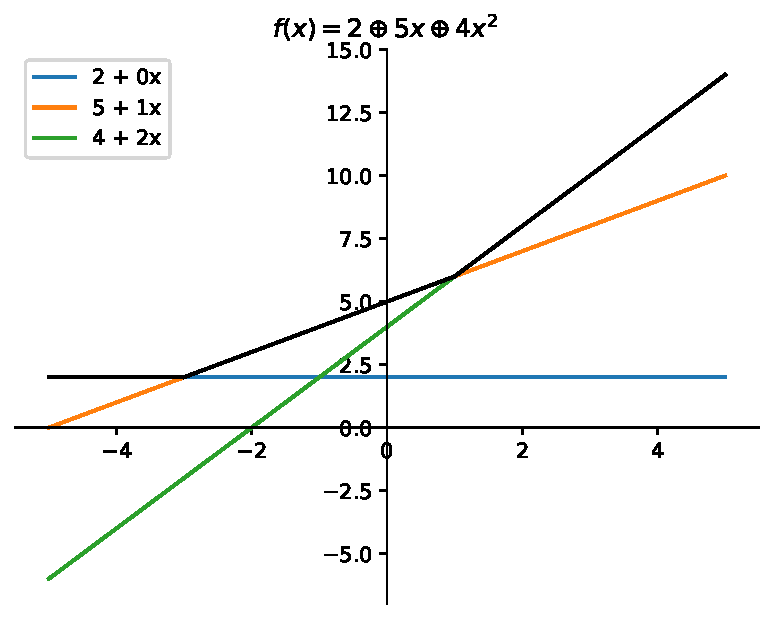
\includegraphics[scale=0.5]{graphics/first_trop_pol.pdf}
\caption{Take $f(x) = 2 \oplus 5x \oplus 4x^{2}$ a quadratic polynomial. The graph equals $max(2, 5+x, 4+2x)$. Until $5-2$, $2$ dominates, from there $5+x$ dominates to the point $4+2x$.}
\label{fig:trop_quad_1}
\end{subfigure}
\begin{subfigure}{0.5\textwidth}
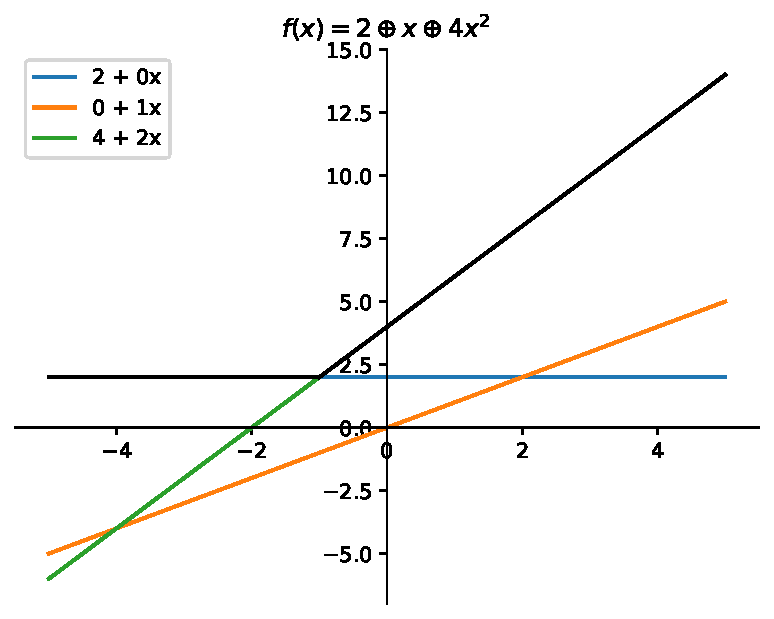
\includegraphics[scale=0.5]{graphics/second_trop_pol.pdf}
\caption{Take $f(x)=2 \oplus x \oplus 4x^{x}$, we have changed the scalar in the second part, then this second part plays no part in the tropical polynomial.}
\label{fig:trop_quad_2}
\end{subfigure}

\caption{Quadratic tropical polynomials.}
\label{fig:image2}
\end{figure}

We can see the degree of a tropical polynomial, defined the same as a degree of a usual polynomial, gives an upper bound for the number of non linear edges of the tropical polynomial, but not the exact value. With higher degree polynomials more non linear edges are possible as figure \ref{fig:trop_qub} illustrates.


\begin{figure}[h]
\centering
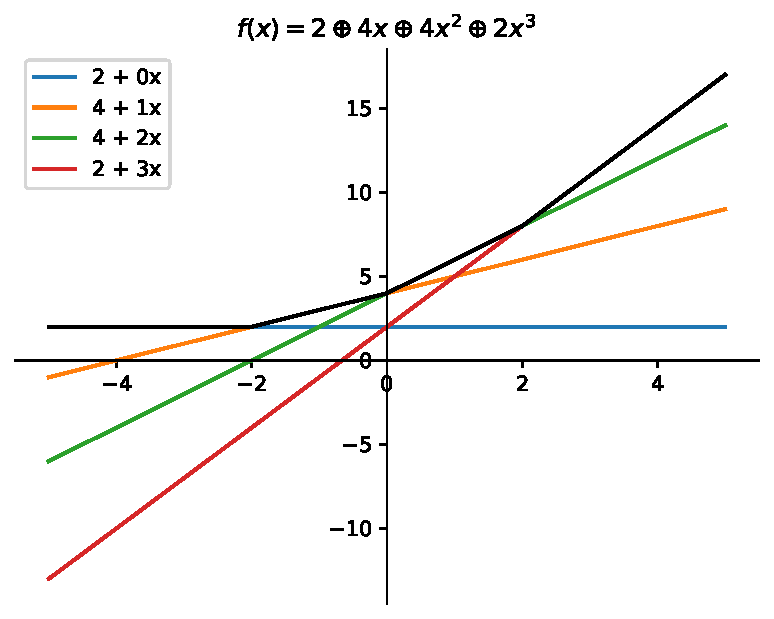
\includegraphics[scale=0.75]{graphics/third_trop_pol.pdf}
\caption{Take $f(x)=2 \oplus x \oplus 4x^{x} \oplus 4x^{2} \oplus 3x^{3}$. For a degree three tropical polynomial in one variable this polynomial has reached the maximum number of non linear edges.}
\label{fig:trop_qub}
\end{figure}
\end{remark}

\begin{definition}
Let $S$ be a set in a real vector space. $S$ is convex if for $s_{1}, s_{2} \in S, \lambda s_{1} + (1-\lambda) S_{2} \in S$ holds with $\lambda \in [0,1] \subset \mathbb{R}$.
\end{definition}

\begin{definition}
Let $X$ be a convex set in a real vector space and let $f:X \to \mathbb{R}$ be a function, then $f$ is called convex if for $x_{1}, x_{2} \in X$ and $\lambda \in [0,1] \subset \mathbb{R}, f(\lambda x_{1} + (1-\lambda)x_{2}) \leq tf(x_{1}) + (1-t)f(x_{2})$ holds.
\end{definition}


\begin{definition}
A function $f : K^{m} \to K^{n}$ with $n, m \in \mathbb{N}$ and $K = \mathbb{R}$ or $K = \mathbb{T}$ is piecewise linear if there exist closed sets $(P_{i})_{i \in \mathbb{N}} \subset K^{n}$ with $f : P_{i} \to K^{n}$ linear and $\cup_{i}P_{i} = K^{m}$.
\end{definition}

In multiple variables we can characterise tropical polynomials as functions from $\mathbb{R}^{n} \to \mathbb{R}$ that satisfy the following three properties.

\begin{lemma}\label{lemma:trop_properties}
Let f be a tropical polynomial
$$ f(x) = c_1^{\alpha_1} \oplus \dots \oplus c_r x^{\alpha_r}$$ as in \ref{tropPolyn}. Then f has three important properties:
\begin{itemize}
\item[(1)]
$f$ is continuous.
\item[(2)]
$f$ is piecewise-linear, where the number of pieces is finite.
\item[(3)]
$f$ is convex, i.e. $p(\frac{x + y}{2}) \leq \frac{1}{2}(p(x)+p(y)) \forall x,y \in \mathbb{R}$
\end{itemize}
\end{lemma}

\begin{proof}
The minimum of continuous functions is still continuous which proves (1). Then every monomial $c_ix^{\alpha_i} = c_i + xy\alpha_{i1} + \dots + x_r \alpha_{ir}$ is per definition linear. Because of (1), linearity can only be broken where $c_i x^{\alpha_i} = c_j x^{\alpha_j}$ for $i \leq j$ and $i,j = 1, \dots ,r$. A piece is a single maximal region of $c_ix^{\alpha_i}$ on which linearity is not broken. If we introduce $c_ix^{\alpha_i}$ one after another, then in the $i$-th step not more than $i^2$ new pieces can be created, so there can only be $ \sum_{i=1}^{r} i^2$ or less pieces which proves (2). 
For (3) let $P_{j}$ be a piece of $f$, where $f(x)=c_{j}x^{\alpha_{j}}$, then with $x_{1} \in P_{j}, \lambda \in [0,1]$ and
\begin{align*}
f(\lambda x_{1} + (1-\lambda)x_{2})
&= c_{j}(\lambda x_{1} + (1-\lambda)x_{2})^{\alpha_{j}} \\
&= c_{j} + \alpha_{j}(\lambda x_{1} + (1-\lambda)x_{2}) \\
&= \lambda(c_{j}+\alpha_{j}x_{1}) + (1-\lambda)(c_{j}+\alpha_{j}x_{2}) \\
&= \lambda f(x_{1}) + (1-\lambda) f(x_{2})
\end{align*}
on one piece f is convex. Moving from one piece $P_{j}$ to another adjacent $P_{i}$ where $f(x)$ is $c_{j}x^{\alpha_{j}}$ and $f(x)=c_{i}x^{\alpha_{i}}$ respectively is modelled by picking $x_{1} \in P_{j}$ and $x_{2} \in P_{i}$ and again proving convexity:
\begin{align*}
f&(\lambda x_{1} + (1-\lambda)x_{2}) \\
&= c_{j}(\lambda x_{1} + (1-\lambda) x_{2})^{\alpha_{j}} \oplus c_{i}(\lambda x_{1} + (1-\lambda) x_{2})^{\alpha_{i}} \\
&= \max \{ c_{j} + \alpha_{j}(\lambda x_{1} + (1-\lambda) x_{2}), c_{i} + \alpha_{i}(\lambda x_{1} + (1-\lambda) x_{2}) \} \\
&= \max \{ \lambda (c_{j} + \alpha_{j}x_{1}) + (1-\lambda) (c_{j} + \alpha_{j}x_{2}) , \lambda (c_{i} + \alpha_{i}x_{1}) + (1-\lambda) (c_{i} + \alpha_{i}x_{2})\} \\
&\leq \max \{ \lambda (c_{j} + \alpha_{j}x_{1}), \lambda (c_{j} + \alpha_{j}x_{1}) \} + \max \{ (1-\lambda) (c_{j} + \alpha_{j}x_{2}), (1-\lambda) (c_{i} + \alpha_{i}x_{2}) \} \\
&= \lambda \max \{ (c_{j} + \alpha_{j}x_{1}), (c_{j} + \alpha_{j}x_{1}) \} + (1-\lambda) \max \{ (c_{j} + \alpha_{j}x_{2}), (c_{i} + \alpha_{i}x_{2}) \} \\
&= \lambda f(x_{1}) + (1-\lambda) f(x_{2})
\end{align*}
which ends the prove.
\end{proof}

\begin{proposition}
Every function $\mathbb{R}^{n} \to \mathbb{R}$ which satisfies the three properties (1), (2) and (3) from lemma 	\ref{lemma:trop_properties} has a representation as the minimum of a finite set of linear functions. Thus, the tropical polynomial in n variables $x_{1}, \dots x_{n}$ represent the class of piecewise-linear convex functions on $\mathbb{R}^{n}$ with integer coefficients.
\end{proposition}

\begin{proof}
This follows directly from lemma \ref{lemma:trop_properties}.
\end{proof}

Now we are ready to introduce tropical rational functions. These are important to understand the core section, section \ref{sec:trop_netw}, in particular the actual connection build between neural networks and tropical geometry in this thesis, as are the semifields $\mathbb{T}[X_{1} , \dots , X_{d}]$ and $\mathbb{T}(X_{1} , \dots , X_{d})$.

\begin{definition} \cite[p.~3]{zhang2018tropical}
Following notations above, a tropical rational function is a standard difference, or, equivalently,
a tropical quotient of two tropical polynomials $f(x)$ and
$g(x)$:
$$ (f-g)(x) = f(x) - g(x) = f(x) \oslash g(x) = (f \oslash g)(x)$$
%We will denote a tropical rational function by $f \oslash g$, where $f$ and $g$ are understood to be tropical polynomial functions.
\end{definition}



\begin{proposition}
$\mathbb{T}[X_1, \dots , X_d] := \{ f: \mathbb{T}^{d} \to \mathbb{T} ; f \ is \ tropical \ polynomial \}$ and \ $ \mathbb{T}(X_1, \dots , X_d) := \{ f: \mathbb{T}^{d} \to \mathbb{T} ; f \ is \ tropical \ rational \ function \}$ are both semifields. \cite[p.~3]{zhang2018tropical}
\end{proposition}
\begin{proof}
Let $g,f,h \in \mathbb{T}(X_1, \dots ,X_d)$ with 
\begin{align*}
f(x) &= f_1(x) \oslash f_2(x) = (\oplus_{i=0}^r c_{1i} x^{\alpha_{1i}}) \oslash (\oplus_{i=0}^r c_{2i} x^{\alpha_{2i}}) \\
g(x) &= g_1(x) \oslash g_2(x) = (\oplus_{i=0}^r d_{1i} x^{\beta_{1i}}) \oslash (\oplus_{i=0}^r d_{2i} x^{\beta_{2i}}) \\
h(x) &= h_1(x) \oslash h_2(x) = (\oplus_{i=0}^r e_{1i} x^{\gamma_{1i}}) \oslash (\oplus_{i=0}^r e_{2i} x^{\gamma_{2i}}) \\
\end{align*}
We begin the proof by showing, that for two tropical polynomials $a(x)= \oplus_{i=0}^r z_{i} x^{\zeta_{i}}), b(x)= \oplus_{i=0}^r o_{i} x^{\omega_{i}}) \in \mathbb{T}[X_1, \dots , X_r]$ the normal sum is a tropical polynomial $(a + b)(x) \in \mathbb{T}[X_1, \dots , X_r]$.
\begin{align*} 
(a + b)(x) &= a(x) + b(x) \\
&=  (\oplus_{i=0}^r z_{i} x^{\zeta_{i}}) + (\oplus_{i=0}^r o_{i} x^{\omega_{i}}) \\
&= \oplus_{i, j = 0, \dots , r} (z_{i} + \zeta_{i} * x + o_{j} + \omega_{i} * x) \\
&= \oplus_{i, j = 0, \dots , r} ((z_{i} + o_{j}) + x^{\zeta_{i} + \omega_{i}}) \in \mathbb{T}[X_1, \dots X_r]
\end{align*}
Other than with the proof of the Tropical semiring we will show that tropical addition and tropical multiplication of tropical polynomials as tropical rational functions stay tropical polynomials respectively tropical rational functions. All other axioms stay pointwise the same.
\begin{itemize}
\item[(1):]
The tropical sum of tropical rational function is a tropical rations function
\begin{align*}
(f \oplus g)(x) &= f(x) \oplus g(x) \\
&=(f_1(x) \oslash f_2(x)) \oplus (g_1(x) \oslash g_2(x)) \\
&= \min\{f_1(x) - f_2(x), g_1(x) - g_2(x) \} \\
&= \min\{f_1(x) + g_2(x), g_1(x) + f_2(x) \} - f_2(x) - g_2(x) \\
&= (f_1(x) + g_2(x) \oplus g_1(x) + f_2(x)) \oslash (f_2(x) + g_2(x)) \in \mathbb{T}(X_1, \dots , X_r).
\end{align*}
since addition as tropical addition of tropical polynomials is a tropical polynomial.
\item[(2):]
The tropical product of tropical rational functions is a tropical rational function
\begin{align*}
(f \odot g)(x) &= f(x) \odot g(x) \\
&=  (f_1(x) \oslash f_2(x)) \odot (g_1(x) \oslash g_2(x)) \\
&= f_1(x) - f_2(x) + g_1(x) - g_2(x) \\
&= (f_1(x) + g_1(x)) - (f_2(x) + g_2(x)) \in \mathbb{T}(X_1, \dots , X_r)
\end{align*}
\item[(3):]
The neutral element for the tropical sum is $- \infty = - \infty \oslash x = x \oslash - \infty \ x \in \mathbb{T}$ since for $f(x) \in \mathbb{T}(X_1, \dots , X_r)$ as above, the following stands $ f(x) \oplus \infty = \max(f(x),\ - \infty) = f(x)$ and with $f(x) \odot 0 = f(x) + 0 = f(x) \forall f(x) \in \mathbb{T}$, $0$ is the neutral element of tropical multiplication.
\end{itemize}
\end{proof}

We regard a tropical polynomial $f=f \oslash 0$ as a special case of a tropical rational function and thus $\mathbb{T}[X_1, \dots , X_r] \subseteq \mathbb{T}(X_1, \dots , X_r)$. \cite[p.~3]{zhang2018tropical}

\begin{comment}
~\
\begin{itemize}
\item[$\bullet$]
A d-variate tropical polynomial $f(x)$ defines a function $f: \mathbb{T}^{d} \to \mathbb{T}$ that is a convex function in the usual sense as taking $\max$ and $\sum$ of convex functions preserve convexity \cite{boyd2004convex}.
\item[$\bullet$]
As such, a tropical rational function $f \oslash g : \mathbb{T}^{d} \to \mathbb{T}$ is a DC function or differenceconvex function \cite{hartman1959functions}.
\end{itemize}
\end{comment}

\begin{definition}
$R : \mathbb{R}^{d} \to \mathbb{R}^{p}, x = (x_1, \dots , x_d)\mapsto (f_1(x), \dots , f_p(x))$, is called a tropical polynomial map if each $f_i : \mathbb{R}^{d} \to \mathbb{R}$ is a tropical polynomial, $i = 1, \dots , p$, and a tropical rational map if $f_1, \dots , f_p$ are tropical rational functions. We will denote the set of tropical polynomial maps by $Pol(d, p)$ and the set of tropical rational maps by $Rat(d, p)$. So $Pol(d, 1) = \mathbb{T}[X_1, \dots , x_d]$ and $Rat(d, 1) = \mathbb{T}(x_1, \dots , x_d)$ \cite[p.~3]{zhang2018tropical}.
\end{definition}

As a logical continuation of chapter \ref{sec:trop_algebra} we choose to introduce tropical hypersurfaces as the \ref{sec:tropical_hypersurfaces}nd chapter. Tropical hypersurfaces will be needed in chapter \ref{sec:tropical_geometry_of_neural_networks} and the end of chapter \ref{sec:trop_netw} exclusively, leading to the fact that there will be a necessary logical gap.

\newpage

%\section{Valuations and tropicalisation}
%
%\begin{definition}\cite[p.~57]{maclagan2015introduction}
%Let $\mathbb{K}$ be a field. We denote by $K^{*}$ the nonzero elements of K. A valuation on $\mathbb{K}$ is a function $val: \mathbb{K} \to \mathbb{R} \cup \{\infty\}$ satisfying the following three axioms:
%\begin{align*}
%1. \ &val(a) = \infty \ \text{if and only if} \ a = 0, \\
%2. \ &val(ab) = val(a) + val(b) \ \text{and} \ \\
%3. \ &val(a + b) \geq \min\{val(a), val(b)\} \ \text{for all} \ a, b \in K^{*}
%\end{align*}
%The image of the valuation map is denoted $\Gamma_{val}$. This is an additive subgroup of the real numbers $\mathbb{R}$ which is called the value group.
%\end{definition}
%\begin{lemma}
%Let $a, b \in \mathbb{K}$. If $val(a) \neq val(b)$ then $val(a+b) = min(val(a), val(b))$.
%\cite[p.~57]{maclagan2015introduction}
%\end{lemma}
%\begin{proof}
%Let $a,b \in \mathbb{K}$. Without loss of generality we may assume that $val(b) > val(a)$. When evaluating $1\in \mathbb{K}$ we observe
%$$val(1)=val(1^{2})=val(1) + val(1)$$
%it follows, that $val(1)=0$, and so $-(1)^{2}$ implies $val(-1)=0$. But with the valuation of $-1$ being zero
%$$val(-b) = val(-1) + val(b) = val(b) \ \text{for all} \ b \in \mathbb{K}$$
%the sign is irrelevant to valuation. The third axiom implies
%$$val(a) \geq \min(a+b), val(-b)) = min(val(a+b), val(b)),$$
%and therefore $val(a) \geq val(a + b)$. But we also have
%$$val(a + b) \geq \min(val(a), val(b)) = val(a),$$
%and hence $val(a + b) = val(a)$ as desired.
%\end{proof}
%\newpage

\section{Tropical hypersurfaces}
\label{sec:tropical_hypersurfaces}

In this chapter we will start viewing tropical polynomials as geometric figures with a surface area that is piecewise linear and boundaries for the number of the linear areas. We hop right in by defining the tropical hypersurface of a tropical polynial. 
 
\begin{definition}\cite[p.~3]{zhang2018tropical}
The tropical hypersurface of a tropical polynomial $f(x) = c_1 x^{\alpha_1} \oplus \dots \oplus c_r x^{\alpha_r}$ is 
$$\Gamma(f) := \{ x \in \mathbb{R}^{d} : c_i x^{\alpha_i} = c_j x^{\alpha_j} = f(x) \ \text{for some} \ \alpha_i \neq \alpha_j \}$$
i.e., the set of points x at which the value of f at x is attained by two or more monomials in f.
\end{definition}

To understand the geometry of tropical rational functions, tropical polynomial maps and tropical rational maps better we will show that each are piecewise linear.


\begin{lemma}
Tropical rational functions are piecewise linear functions. Tropical polynomial maps and tropical rational maps are piecewise linear maps.
\end{lemma}
\begin{proof}
Because of \ref{lemma:trop_properties} tropical polynomials are piecewise linear. $\oslash$ is a linear transformation, therefore the tropical rational maps are piecewise linear two. Now this means that tropical rational maps and tropical polynomial maps are also piecewise linear and the notion of linear regions applies.
\end{proof}

\begin{definition}
A linear region of $F \in Rat(d, m)$ is a maximal connected subset of the domain on which $F$ is linear. The number of linear regions of $F$ is denoted $\mathcal{N}(f)$ \cite[p.~4]{zhang2018tropical}.
\end{definition}

The linearity of a tropical polynomial per definition will be broken on its hypersurface and linear everywhere else. Therefore the tropical hypersurface $\Gamma(f)$ of a tropical polynomial $f$ divides the domain of f into convex cells on each of witch f is linear.

\begin{definition}\cite[p.~3]{zhang2018tropical}
Tropical hypersurfaces of polynomials in two variables are called tropical curves.
\end{definition}

\begin{definition}\cite[p.~3]{zhang2018tropical}
The Newton polygon of a tropical polynomial $f(x) = c_1 x^{\alpha_1} \oplus \dots \oplus c_r x^{\alpha_r}$  is the convex hull of $\alpha_1 , \dots , \alpha_r \in \mathbb{N}^{d}$, regarded as points in $\mathbb{R}^{d}$,
$$ \Delta(f) := Conv{\alpha_i \in \mathbb{R}^{d} : c_i \neq -\infty , i = 1, \dots ,r } $$.
\end{definition}

\begin{comment}\cite[p.~3]{zhang2018tropical}
A tropical polynomial $f$ determines a dual subdivision of
$\delta (f)$, constructed as follows. First, lift each $\alpha_i$ from $\mathbb{R}^d$ into $\mathbb{R}^{d+1}$ by appending $c_i$ as the last coordinate. Denote the convex hull of the lifted $\alpha_1, \dots , \alpha_r$ as
$$\mathcal{P}(f):= Conv{(\alpha_i, c_i) \in \mathbb{R}^{d} \times \mathbb{R} : i = 1, \dots , r}. (1)$$
Next let $UF(\mathcal(P)(f))$ denote the collection of upper faces in $\mathcal{P}(f)$ and $\pi : \mathbb{R}^{d} \times \mathbb{R} \to \mathbb{R}^{d}$ be the projection that drops
the last coordinate. The dual subdivision determined by $f$
is then
$$\delta(f) := {\pi(p) \subset \mathbb{R}^{d} : p \in UF( \mathcal{P}(f))}.$$.
$\delta (f)$ forms a polyhedral complex with support $\delta (f)$. By \cite{maclagan2015introduction}, the tropical hypersurface $\mathcal{T}(f)$ is the $(d - 1)$-skeleton of the polyhedral complex dual to $ \delta(f)$. This means that each vertex in $ \delta(f)$ corresponds to one "cell" in $R^{d}$ where the function f is linear. Thus, the number of vertices in $\mathcal{P}(f)$ provides an upper bound on the number of linear regions of $f$.
\end{comment}

Our analysis of neural networks will require figuring out
how the polytope $\mathcal(P)(f)$ transforms under tropical power,
sum, and product.

\begin{proposition}\cite[p.~4]{zhang2018tropical}
Let $f$ be a tropical polynomial and let $a \in \mathbb{N}$. Then
$$ \mathcal{P}(f^{a}) = a \mathcal{P}(f) $$.
$a \mathcal{P}(f) = \{ax : x \in \mathcal{P}(f) \} \subset \mathbb{R}^{d + 1}$ is a scaled version of $\mathcal{P}(f)$ with the same shape but different volume.
\end{proposition}
\begin{proof}
Let $f(x)=c_{1}x^{\alpha_1} \oplus \dots \oplus c_{r}x^{\alpha_r}, f:\mathbb{T}^{n} \to \mathbb{T}$, as in \ref{tropPolyn}. Then with $\mathcal{P}(f) = Conv\{(\alpha_{i}, c_{i}) \in \mathbb{R}^{d} \times \mathbb{R}, i= 1, \dots , r and c_{i} \neq - \infty \}$.
\begin{align*}
f^{a} &= (c_{1}x^{\alpha_{1}} \oplus \dots \oplus c_{r} x^{\alpha_{r}})^{a} \\
&= a \cdot (c_{1}x^{\alpha_{1}} \oplus \dots \oplus c_{r} x^{\alpha_{r}}) \\
&= a \cdot (c_{1}x^{\alpha_{1}}) \oplus \dots \oplus a \cdot (c_{r} x^{\alpha_{r}}) \\
&= (a \cdot c_{1})x^{a \cdot \alpha_{1}} \oplus \dots \oplus (a \cdot c_{r}) x^{a \cdot \alpha_{r}}
\end{align*}
and therefore
$$\mathcal{P}(f^{a}) = Conv\{(a \cdot \alpha_{i}, a \cdot c_{i}) \in \mathbb{R}^{d} \times \mathbb{R}, i = 1, \dots, r \ \text{and} \ c_{i} \neq - \infty \} = a\mathcal{P}(f)$$.
\end{proof}

A generalisation of normal summation, now on sets, is the Minkowski sum.

\begin{definition}\cite[p.~4]{zhang2018tropical}
The Minkowski sum of two sets $P_1$ and $P_2$ in $\mathbb{R}^{d}$ is the set
$$ P_1 + P_2 := \{x_1 + x_2 \in \mathbb{R}^{d} : x_1 \in P_1 ,x_2 \in P_2 \} $$;
and for $\lambda_1 , \lambda_2 \geq 0$, their weighted Minkowski sum is
$$ \lambda_1 P_1 + \lambda_2 P_2 := \{ \lambda_1 x_1 + \lambda_2 x_2 \in \mathbb{R}^{d} : x_1 \in P_1 , x_2 \in P_2 \} $$.
\end{definition}

One important example for an Minkowski sum is a zonotope. For that we need a notion of the following.
\begin{definition}
A subset $A \subset \mathbb{V}$ of a vector field $\mathbb{V}$ is a line segment, if $A=\{\lambda x + \lambda (1-y) \ | \ \lambda \in [0,1]\subset \mathbb{K}\}$ with $\mathbb{K}$ being the scalar field of $\mathbb{V}$.
\end{definition}

\begin{definition}\cite[p.~4]{zhang2018tropical}
The Minkowski sum of line segments is called a zonotope.
\end{definition}

\begin{definition}
\label{def:dot_sym}
Let $A \subset \mathbb{R}^{n}$ be a set. A is dot symmetric around $b \in A$ if for $a \in A$ follows $a + 2(b-a)=2b-a \in A$
\end{definition}

Obviously for $A$ and $b$ as in \ref{def:dot_sym} and $A$ is convex, then $b \in A$ the symmetry point must lie in $A$. We get an intuition of zonotopes by proving the following statement.

\begin{lemma}
\label{lem:zon_sym_conv}
A zonotope over $\mathbb{R}^{n}$ is dot symmetric and convex.
\end{lemma}
\begin{proof}
We proof a zonotope is dot symmetric and convex by induction. As base case let $P \subset \mathbb{R}^{n}$ be a line segment in between $x, y \in \mathbb{R}^{n}$ then $P$ is obviously dot symmetric around $b=0.5(x+y) \in \mathbb{R}^{n}$ and convex per definition. For the induction step let $A \subset \mathbb{R}^{n}$ be a convex set and dot symmetric around $b \in \mathbb{R}^{n}$ and also let $P = \{ \lambda x + (1- \lambda) y | \lambda \in [0,1] \subset \mathbb{R}^{n} \}$ for $x, y \in \mathbb{R}^{n}$. Then the Minkowski sum of the two sets is
\begin{align*}
A + P 
&= \{ a + p | a \in A \ \text{and} \ p \in P \} \\
&= \{ a + \lambda x + (1- \lambda) y | a \in A \ \text{and} \ \lambda \in [0,1] \}
\end{align*}
It follows that $a_{A+P} \in A+P$ has the form $a_{A+P}=a + \lambda x + (1- \lambda)y$ for $a\in A$ and $\lambda \in [0,1]$. We set $b_{A+P}=(0.5)(x+y) + b$. Then
\begin{align*}
a_{A+P} + &2(b_{A+P} - a_{A+P}) \\
&= a + \lambda x + (1- \lambda)y + 2( 0.5(x+y) + b - (a + \lambda x + (1-\lambda)y)) \\
&= 2b-a + (1- \lambda) x + \lambda y \in A+P
\end{align*}
since $2b-a \in A$ and $(1- \lambda) x + \lambda y \ in P$. Therefore a zonotope is symmetric.
Similarly for convexity let $p, q \in A+P$ have the shape
\begin{align*}
p &= a_{p} + \lambda_{p} x + (1 - \lambda_{p}) y \\
q &= a_{q} + \lambda_{q} x + (1 - \lambda_{q}) y.
\end{align*}
For $\mu \in [0, 1] \subset \mathbb{R}^{n}$ we need to compute
\begin{align*}
\mu p + (1 - \mu) q &= \mu (a_{p} + \lambda_{p} x + (1-\lambda_{p}) y) + (1-\mu)(a_{q} + \lambda_{q} x + (1-\lambda_{q}) y) \\
&= \mu a_{p} + (1-\mu) a_{q} + (\mu \lambda_{p} + (1-\mu)\lambda_{q})x + (\mu(1-\lambda_{p}) + (1-\mu)(1-\lambda_{q}))y \\
&= \mu a_{p} + (1-\mu) a_{q} + \Phi x + (1- \Phi) y
\end{align*}
with $\Phi = \Phi(\mu , \lambda_{p}, \lambda_{q}) = \mu \lambda_{p} + \lambda_{q} - \mu \lambda_{q}$. If $0 \leq \Phi (\mu, \lambda_{p}, \lambda_{q}) \leq 1$, then a zonotope would be convex, since $(1-\mu) a_{q} + \Phi x + (1- \Phi) y \in P$ would hold and $\mu a_{p} + (1-\mu) a_{q} \in A$ holds anyway. So to conclude we show $0 \leq \Phi (\mu, \lambda_{p}, \lambda_{q}) \leq 1$. \
Because of $\mu \lambda_{p} \geq 0$ and $\lambda_{q} \geq \mu \lambda_{q}$ follows $\Phi \geq 0$. $\Phi$ is maximal for $\lambda_{p} = 1$ and $\Phi (\mu, 1, \lambda_{q}) = \mu + \lambda_{q} - \mu \lambda_{q} \leq 1$.
\end{proof}

Let $\mathcal{V}$ denote the set of vertices of a polytope $P$. Clearly, the Minkowski sum of two polytopes is given by the convex hull of the Minkowski sum of their vertex sets, i.e., $P_{1} + P_{2} = Conv(\mathcal{V}(P1) + \mathcal{V}(P2))$. With this observation, the
following is immediate.

\begin{proposition} \cite[p.~4]{zhang2018tropical}
Let $f, g \in Pol(d, 1) = \mathbb{T}[x_1, \dots , x_d]$ be tropical polynomials. Then
\begin{align*}
\mathcal{P}(f \odot g) &= \mathcal{P}(f) + \mathcal{P}(g), \\
\mathcal{P}(f \oplus g) &= Conv(\mathcal{V}(\mathcal{P}(f)) \cup \mathcal{V}( \mathcal{P}(g))).
\end{align*}
\end{proposition}

We reproduce below part of \cite[Theorem 2.1.20]{gritzmann1993minkowski} and derive a corollary for bounding the number of verticies on the upper faces of a zonotope.

\begin{theorem}
\label{theo:gritzmann_sturmfels}
\cite{gritzmann1993minkowski}. Let $P_1, \dots , P_k$ be polytopes in $\mathbb{R}^{d}$ and let m denote the total number of nonparallel edges of $P_1, \dots , P_k$. Then the number of vertices of $P_1 + \dots + P_k$ does not exceed
$$\sum_{j=0}^{d-1} \binom{m-1}{j}.$$
The upper bound is attained if all $P_i$'s are zonotopes and all their generating line segments are in general positions.
\end{theorem}

And now we come to the main corollary of this chapter, core to chapter \ref{sec:tropical_geometry_of_neural_networks}.

\begin{corollary}\cite[p.~4]{zhang2018tropical}
Let $\mathcal{P} \in \mathbb{R}^{d+1}$ be a zonotope generated by m line segments $P_1 , \dots , P_m$. Let $\pi : \mathbb{R}^{d} \times \mathbb{R} \to \mathbb{R}^{d}$ be the projection. Suppose $P$ satisfies:
\begin{itemize}
\item[(i)]
the generating line segments are in general positions;
\item[(ii)]
the set of projected vertices $\{ \pi(v) : v \in \mathcal{V}(\mathcal{P}) \} \subseteq \mathbb{R}^{d}$ are in generalposition.
\end{itemize}
Then $P$ has
$$ \sum_{j=0}^{d} \binom{m}{j} $$
vertices on its upper faces. If either (i) or (ii) is violated, then this becomes an upper bound.
\end{corollary}
\begin{proof}
Let $V_{1}$ be the vertices of the upper and $V_{2}$ the vertices of the lower face of P in relation to the projection $\pi$. As a consequence of (i), $P_{1}, \dots , P_{k}$ are nonparallel and with \ref{theo:gritzmann_sturmfels} follows the number of vertices of $\mathcal{P}$ is 
$$n_{1} = 2 \sum^{d}_{j=0} \binom{m-1}{j}.$$ 
Because a zonotope is convex \ref{lem:zon_sym_conv} the upper and lower faces of P must already be all faces and $|V_{1} \cup V_{2}| = n_{1}$ holds. Also because of \ref{lem:zon_sym_conv}, zonotopes are symmetric and therefore $|V_{1}| = |V_{2}|$ the upper and lower faces are of same cardinality. Let $P' := \pi (P)$ be the projection of $P$ in $\mathbb{R}^{d}$. (ii) would not hold if $\pi(P_{1}), \dots , \pi(P_{2})$ where not in general position and therefore $P'$ is generated by m line segments and $P'$ has 
$$n_{2}=2 \sum^{d-1}_{j=0} \binom{m-1}{j}$$
vertices, since the dimension has gone one lower. For any vertex $v \in P$, if $v \in V_{1} \setminus V_{2} \cup V_{2} \setminus V_{1}$ then $v$ can not be a vertex of $P'$ since all of these get dropped by the projection. On the other hand $v \in (V_{1} \cup V_{2}) \setminus (V_{1} \setminus V_{2} \cup V_{2} \setminus V_{1}) = V_{1} \cap v_{2}$ can not get dropped by the projection of $P$ and therefore the number of vertices on $P'$ equals $|V_{1} \cap V_{2}|$, thus $n_{2} = |V_{1} \cap V_{2}|$ and we can calculate the number of vertices on the upper face of $P$:
\begin{align*}
|V_{2}|
&= 0.5(|V_{1} \cup V_{2}| - |V_{1} \cap V_{2}|) + |V_{1} \cap V_{2}| \\
&= 0.5(n_{1} - n_{2}) + n_{2} \\
&= 0.5(2 \sum^{d}_{j=0} \binom{m-1}{j} - 2 \sum^{d-1}_{j=0} \binom{m-1}{j}) + 2 \sum^{d-1}_{j=0} \binom{m-1}{j} \\
&= \binom{m-1}{d} + 2 \sum^{d-1}_{j=0} \binom{m-1}{j} \\
&= \sum^{d}_{j=0}(\binom{m-1}{j} + \binom{m-1}{j-1}) \\
&= \sum^{d}_{j=0} \binom{m}{j}
\end{align*}
\end{proof}

\newpage

\section{Neural networks}
\label{sec:neural_networks}
Neural networks viewed as a topic, make for a very compelling field of interest in their own right. Historically the term "Neural Network" was introduced in attempts to describe the functionality of biological processes, in particular the nervous system and the brain, in a mathematical sense \cite{mcculloch1943logical, widrow1960adaptive, rumelhart1986learning}. Simplified the nervous system is a net of neurons, each having a soma and an axon. At any instant a neuron has some threshold, which excitation must exceed to initiate an impulse. This, except for the fact and the time of its occurrence, is determined by the neuron, not by the excitation. From the point of excitation the impulse is propagated to all parts of the neuron \cite{mcculloch1943logical}. Through synapses the axons are connected to further soma through which the impulse is passed on to further neurons. Impulses passing through the nervous system partly consist of electrical impulses and chemical reactions \cite{palay1956synapses}. A collection of partially connected neurons, capable of carrying impulses, is called a biological neural network.


\begin{figure}[H]
\centering
\figuretitle{Depiction of a neuron}
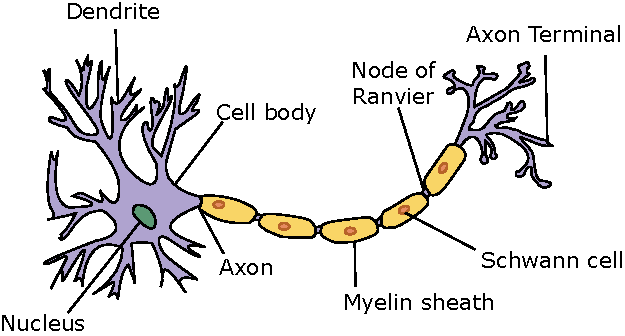
\includegraphics[scale=0.75]{graphics/neuron.pdf}
\caption{A representation of a neuron. The axon terminal attach to dendrite. This way impulses pass from neuron to neuron.}
\label{fig:neuron}
\end{figure}

In reference to a biological neural network, an abstract neuronal network, in the following simply referenced as neuronal networks, are defined. As a biological neuron and especially a biological neural network are far more complex than this introduction may make it seem, biological realism would impose entirely unnecessary constraint. Boiling a biological neuronal network down to its quintessential features results in a weighted directed graph, where edges and vertices are weighted. Typically a weighted graph only has its edges weighted. To fit our model better we introduce them also with weighted vertices.

\begin{definition}
A graph is a pair $G = (V, E)$, where $V$ is a set whose elements are called vertices, and $E \subset \{ {x, y}|(x,y) \in v^{2} \}$ is a set of two-sets of vertices, whose elements are called edges.
\end{definition}

\begin{definition}
A directed graph is a pair $G = (V, E)$, where $V$ is a set whose elements are called vertices, and $E \subset \{ (x, y)|(x,y) \in v^{2} \}$ is a set of edges which are ordered pairs of distinct vertices.
\end{definition}

\begin{definition}
A weighted graph $G = (V, E)$ in our case is attributed by two functions $\psi : V \to \mathbb{K}$ and $\omega : E \to \mathbb{K}$ that assign a weight $\psi(v)$ and $\omega(e)$ to each edge $e \in E$ and weight $v \in V$, with $\mathbb{K}$ being a field.
\end{definition}

\begin{definition}
Let $G = (V, E)$ be a Graph. We set $n(G) = |V|$ to be the cardinality of vertices and $m(G) = |E|$ the cardinality of edges.
\end{definition}

Graphs can represent a multitude of relations between objects. Like road maps of roads connecting cities. Or describe objects themselves like molecules.

\begin{remark}
For instance the following weighted directed Graph could depict a road map with cities as nodes connected by roads that are weighted with the distance between cities and we want to find the minimal distance from any city to city A. \

\begin{figure}[H]
\centering
\figuretitle{Min distance weighted graph}
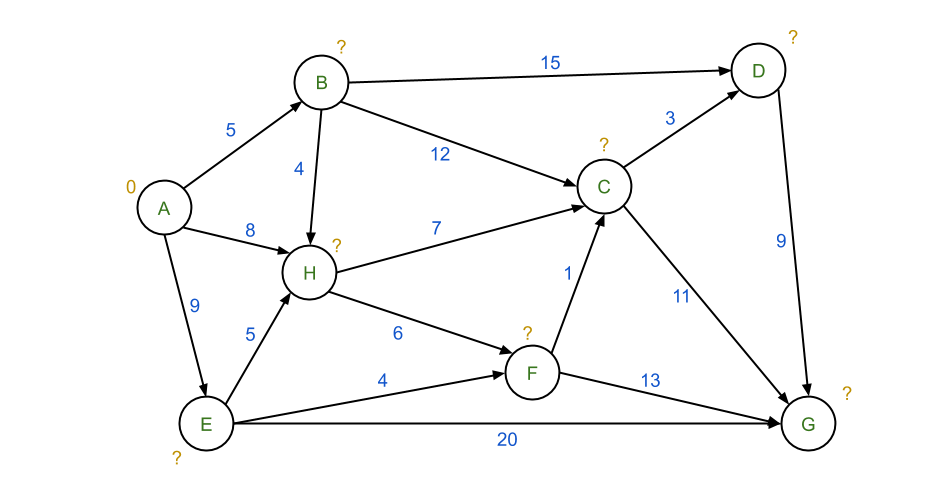
\includegraphics[scale=0.5]{graphics/weighted_directed_graph_2.png}
\caption{Min distance weighted graph.}
\label{fig:neuron}
\end{figure}

In a graph where we have a way to reach each node from the starting point, as our graph has this property, Dijkstra's algorithm gives us, for small graphs, an easy algorithm to compute the shortest path from node A to any other node by hand. At any point in the algorithm simply consider all reachable nodes from nodes that have their shortest path already computed by adding up the shortest paths length to the previous node and the path length of the path between the nodes. This way every reachable node by nodes with there shortest path already computed get at least one or multiple lengths of paths assigned to them. Pick the shortest path under all of these and repeat until all vertices have a path assigned. If there are multiple shortest paths, pick one of them. \\
We will proof that this gives us a correct result through induction.
\begin{proof} 
For each node $v$, $dist(v)$ is the shortest distance from source to $v$ when travelling via visited nodes only, or infinity if no such path exists. (Note: we do not assume $dist(v)$ is the actual shortest distance for unvisited nodes.) \\
The base case is when there is just one visited node, namely the initial node source, in which case the hypothesis is trivial. \\
Otherwise assume the hypothesis for $n-1$ visited nodes, n which case we choose an edge $vu$ where $u$ has the least $dist(u)$ of any unvisited nodes and the edge $vu$ is such that $dist(u) = dist(v) + length(v,u)$. $dist(u)$ is considered to be the shortest distance from source to $u$ because if there were a shorter path, and if $w$ was the first unvisited node on that path then by the original hypothesis $dist(w) > dist(u)$ which creates a contradiction. Similarly if there were a shorter path to u without using unvisited nodes, and if the last but one node on that path were $w$, then we would have had $dist(u) = dist(w) + length(w,u)$, also a contradiction. \\
After processing $u$ it will still be true that for each unvisited node $w$, $dist(w)$ will be the shortest distance from source to $w$ using visited nodes only, because if there were a shorter path that doesn't go by $u$ we would have found it previously, and if there were a shorter path using u we would have updated it when processing $u$. \\
After all nodes are visited, the shortest path from source to any node $v$ consists only of visited nodes, therefore $dist(v)$ is the shortest distance.
\end{proof}

Now that we understand Dijkstra's algorithm, to complete the remark, we will compute the shortest distance to vertex $C$, by terminating Dijkstra's algorithm as soon as we have computed the shortest path to $C$. \\
From $A$ the shortest distance to adjacent vertices is the distance to vertex $B$ with length $5$. We set the shortest distance to $B$ to $5$ and repeat. This time we have to also consider the the distances to adjacent vertices to $B$ with the added shortest distance to $B$. So in this iteration paths of length $20$ to $D$, $17$ to $C$ and $9$ to $H$ with is closely beaten by $8$ to $H$ from $A$ are to be considered. We mark $8$ to be the shortest distance to $H$. We describe one more step in detail and let the reader confirm if the calculated value for $C$ is correct. We have now computed the minimal distance to nodes $A$, $B$ and $H$. Reachable nodes at this point are $D$, $C$, $F$ and $E$ with path lengths of $20, 17, 15, 14$ and $9$. $9$ is the shortest, the shortest way to node $E$ is of length $9$. Next is node $F$ and then $C$ with it's length being $14$.

\end{remark}

Graph theory is a big field, but we are interested in modelling neural networks. In particular in those neural networks that have specific input layers and output layers. Our goal at this point is to get an insight of how to construct a neural network and define weights, so that our output stands in a predefined relation to our input.
In particular one of the most important neural networks is the L-layer feedforward neural network. \
We will define and motivate L-layer feedforward neural networks using graphs at first and then abstract again to only their necessary features.

\begin{definition}
An $L$-layer feedforward neural network in graph form $(G, \sigma)$ is a weighted graph $G=(V, E)$ with an activation function $\sigma: \mathbb{R} \to \mathbb{R}$. $\sigma$ needs to be piecewise differentiable. The graph consists of $L$ sets $V^{(j)}$, $j = 1, \dots , L$ of vertices $(V=\cup_{j=1}^{L}V^{(j)})$ with $L-1$ corresponding sets of edges $E^{(i)} \subset \{(x,y)|x \in V^{(i)}; y \in V^{(i+1)}\}$, $i = 1, \dots , L-1$ which connect two consecutive layers.
\end{definition}

The Graph of a $0$-layer feedforward neural network is an empty graph and of a $1$-layer feedforward neural network is a set of vertices without connecting edges. $\sigma$ will be applied in between propagating nodes in forward propagation \ref{def:forward_propagation}.

\begin{remark}
The first layer of an $L$-layer feedforward neural network is called the input layer and the last ($L$-th) layer is called the output layer. All layers in between collectively are called hidden layers.
\end{remark}

\begin{remark}
A fully connected feedforward neural network $(G, \sigma)$ with $G = (V, E)$ is one where $E$ is the largest out of every possible sets of $E$. This will give the unique solution, where $V^{(j)}$ and $V^{(j+1)}$ for each $j = 1, \dots , L-1$ will be fully connected.
\end{remark}

We are at an interesting point of this chapter. Inspired by biological neural networks, which are the core building blocks of animal brains, we have abstracted some of the essential features, given an introduction to graphs and used these as a mathematical buildingblock for neural networks.
With the introduction of feedforward neural networks we have cast a sensible form of neural network which is able to store and also learn complex relations between input data and output data through forward and backward propagation. \\
Forward propagation describes the process by which from an input vector the output vector is calculated. First we need to introduce the bias and weight vector $W^{(j)}$.

\begin{remark}\label{standardGraphLabeling}
Let $(G, \sigma)$ be a $L$-layer feedforward neural network where we fixate the elements from the sets $V^{(j)}$, by naming them $b_{j1}$ to $b_{j|V^{(j)}|}$, so that we can establish a correlating vector $b^{(j)} = (b_{j1}, \dots ,b_{j|V^{(j)}|})^{t}$, we call this vector the bias of layer $j$, which corresponds to the weights of vertices in $V^{(j)}$ for $j = 2, \dots , L$ and a matrix $W^{(j)}$ with the entries $W^{(j)}_{nm} = \omega((b_{j-1n}, b_{jm}))$ which correspond to the weights of edges connecting layer $j-1$ and $j$ where $j$ is still in range $j = 2, \dots , L$.
\end{remark}

We will label feedforward neural networks this way until we define feedforward neural networks as functions and are now in a position to define forward propagation.

\begin{definition}(Forward Propagation)
\label{def:forward_propagation}
Let $(G, \sigma)$ be as in \ref{standardGraphLabeling}. A Forward Propagation of our $L$-layer feedforward neural network $(G, \sigma)$ and an input vector x, corresponds to the value of $a^{(L)}$, where $z^{(j)} = W^{(j)} a^{(j-1)} + b^{(j)}$, $a^{(j)} = \sigma(z^{(j)})$, for $j=2, \dots , L$ and $a^{(1)} = x$.
\end{definition}

\begin{wrapfigure}{r}{0.5\textwidth}
\centering
%\figuretitle{Min distance weighted graph}
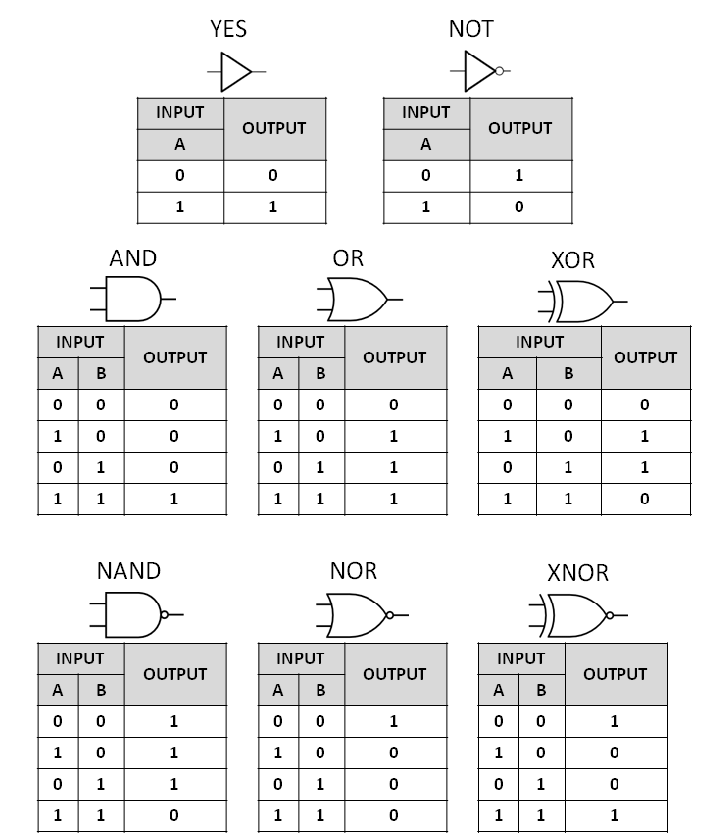
\includegraphics[scale=0.2]{graphics/Summary-of-the-common-Boolean-logic-gates-with-symbols-and-truth-tables.png}
\caption{Boolean Gates Truth Tables}
\label{fig:bool_gate}
\end{wrapfigure}

Often binary inputs, as for example black and white pictures, are fed into neural networks and binary outputs, like dogs or cats are expected. For the sake of proving that the feedforward neural networks we have defined are able to be set up, so that for any specific binary input any binary specific output can be obtained. We will view the infrastructure of the weights, bias and the function $\sigma$ together as a circuit. 

\begin{remark}
Binary circuits are defined by basic logical gates like AND, OR, and NOT gates and a lot more, that manipulate binary input as shown in figure \ref{fig:bool_gate}. A set of gates is called a Universal Logic Gates Set if with those gates any other logic or boolean function can be created. After \cite{quine1955way} AND, OR and NOT define such a set. Meaning if we can reproduce these three gates in form of feedforward neural networks, any boolean logic can be created by these. For that we set $\omega=\mathds{1}$, the weights of edges to one and
\[ \sigma(x) = 
  \begin{cases}
    1       & \quad \text{if } x > 0\\
    0  		& \quad \text{if } x \leq 0.
  \end{cases}
\]
%Then again NAND and NOR both can make a AND, OR and NOT gait, so ether of them are so called minimal universal logic gates, meaning they can make any other logic of Boolean function on their own.
Usually the output of a neural network is non binary, but is trained so that the higher the output value is the higher the probabillity of the specific outcome and the lower the output the lower the probability, with zero being neutral. To skip this interpretation $\sigma$ is defined to immediately produce a binary output. Now we will define three different $2$-layer feedforward neural nets with this sigma.


\begin{figure}[H]
    \centering
    \begin{subfigure}[b]{0.3\textwidth}
        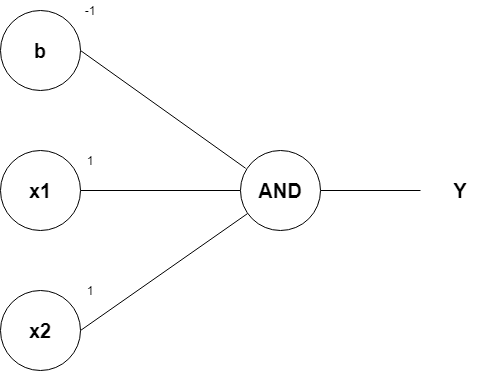
\includegraphics[width=\textwidth]{graphics/AND_gate.png}
        \caption{AND gate}
        \label{fig:AND}
    \end{subfigure}
    \begin{subfigure}[b]{0.3\textwidth}
        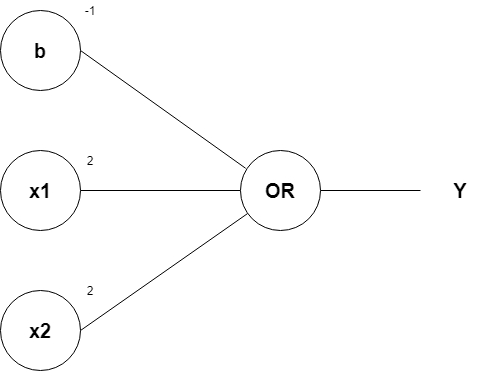
\includegraphics[width=\textwidth]{graphics/OR_gate.png}
        \caption{OR gate}
        \label{fig:OR}
    \end{subfigure}
    \begin{subfigure}[b]{0.3\textwidth}
        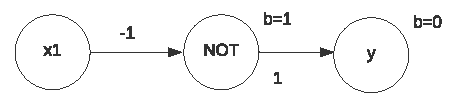
\includegraphics[width=\textwidth]{graphics/NOT_gate.png}
        \caption{NOT gate}
        \label{fig:NOT}
    \end{subfigure}
    \caption{Neural Logical Gates}\label{fig:neural_logic_gates}
\end{figure}
The first, motivated by figure \ref{fig:neural_logic_gates} (a), defines our AND gate. It is defined with the graph $G=(E, V)$, $V=\{ b_{11}, b_{12}, b_{21}, b_{31} \}$, $E=\{ (b_{11}, b_{21}), (b_{12}, b_{21}), (b_{21}, b_{31})\}$ a fully connected neural network with weights 
$$\psi(b_{11})=\psi(b_{12})=\psi(b_31)=0, \ \psi(b_{21})=-1 \ and \ W^{(1)}=\begin{pmatrix}1\\1\end{pmatrix}, \ W^{(2)}=\begin{pmatrix}1\end{pmatrix}.$$
Lets compare the the boolean output with the truth table. Inputs $\{(x, y)|x, y \in \{0, 1\}\}$ with
$$z^{(1)}=(1, 1)\begin{pmatrix}x\\y\end{pmatrix}-1 \ \to \ z^{(2)} = (1)(\sigma(x+y-1))+0 = \sigma(x+y-1)$$
\begin{align*}
for \ (0, 0) \ yield \ z^{(2)}&=\sigma(-1)=0 \\
for \ (1, 0), (0, 1) \ yield \ z^{(2)}&=\sigma(0)=0 \\
and \ for \ (1, 1) \ yield \ z^{(2)}&=\sigma(1)=1.
\end{align*}
The same graph with weights
$$\psi(b_{11})=\psi(b_{12})=\psi(b_31)=0, \ \psi(b_{21})=-1 \ and \ W^{(1)}=\begin{pmatrix}2\\2\end{pmatrix}, \ W^{(2)}=\begin{pmatrix}1\end{pmatrix}$$
makes an OR gate:
$$z^{(1)}=(2, 2)\begin{pmatrix}x\\y\end{pmatrix}-1 \ \to \ z^{(2)} = (1)(\sigma(2x+2y-1))+0 = \sigma(2x+2y-1)$$
\begin{align*}
for \ (0, 0) \ yield \ z^{(2)}&=\sigma(-1)=0 \\
for \ (1, 0), (0, 1) \ yield \ z^{(2)}&=\sigma(2)=1 \\
and \ for \ (1, 1) \ yield \ z^{(2)}&=\sigma(4)=1.
\end{align*}
And last but not least the graph of the NOT gate is different in that it only has one input. Therefore the graph also changes to $G=(E, V)$, $V=\{ b_{11}, b_{21}, b_{31} \}$, $E=\{ (b_{11}, b_{21}), (b_{21}, b_{31})\}$ also a fully connected $2$ feedforward neural network. With weights
$$\psi(b_{11})=\psi(b_31)=0, \ \psi(b_{21})=1 \ and \ W^{(1)}=(-1), \ W^{(2)}=(1)$$
that define a NOT gate:
\begin{align*}
for \ (0) \ yield \ z^{(2)}&= z^{(1)} = 1 \\
and \ for \ (1) \ yield \ z^{(2)}&= z^{(1)} = 0.
\end{align*}

We have proven that any binary input can create any binary output. This also means that by scaling the input and output weights it is possible from any specific input to create any specific output.

\end{remark}

The last abstraction level of feedforward neural networks is to define them as a function, which enables to us to compare feedforward neural networks to tropical polynomials in Chapter $4$.

\begin{definition}\cite{zhang2018tropical}
Viewed abstractly, an L-layer feedforward neural network is a map $\nu : \mathbb{R}^{d} \to \mathbb{R}^{p}$ given by a composition of functions
$$ \nu = \sigma^{(L)} \circ \rho^{(L)} \circ \sigma^{(L-1)} \circ \rho^{(L-1)} \circ \dots \circ \sigma^{(1)} \circ \rho^{(1)}$$
The preactivation functions $\rho^{(1)}, \dots , \rho^{(L)}$ are affine transformations to be determined and the activation functions $\sigma^{(1)}, \dots , \sigma^{(L)}$ are chosen and fixed in advanced. \\
We denote the width, i.e., the number of nodes, of the $l$th
layer by $n_l, l = 1, \dots , L-1$. We set $n_0 := d$ and $n_L := p$, respectively the dimensions of the input and output of the network. The output from the lth layer will be denoted by
$$\nu = \sigma^{(l)} \circ \rho^{(l)} \circ \sigma^{(l-1)} \circ \rho^{(l-1)} \circ \dots \circ \sigma^{(1)} \circ \rho^{(1)}$$
i.e., it is a map $\nu^{(l)} : \mathbb{R}^{d} \to \mathbb{R}^{n_l}$. For convenience, we assume $\nu^{(0)}(x) := x$. \\
The affine function $\nu^{(l)} : \mathbb{R}^{n_{l-1}} \to \mathbb{R}^{n_{l}}$ is given by a weight matrix $A^{(l)} \in \mathbb{Z}^{n_l \times n_{l-1}} $ and a bias vector $b^{(l)} \in \mathbb{R}^{n_l}$:
$$ \rho^{(l)}(\nu^{(l-1)}) := A^{(l)} \nu{(l-1)} + b^{(l)}. $$
The $(i, j)$th coordinate of $A^{(l)}$ will be denoted $a^{l}_{ij}$ and the $i$th coordinate of $b^{(l)}$ by $b^{(l)}_{i}$. Collectively they form the parameters of the $l$th layer
\end{definition}

This way forward propagation corresponds to evaluation of the neural network.

\begin{comment}\cite{zhang2018tropical}
For a vector input $x \in \mathbb{R}^{n_l}, \sigma^{(l)}(x)$ is understood to be in coordinatewise sense; so $\sigma : \mathbb{R}^{n_l} \to \mathbb{R}^{n_l}$. We assume the
final output of a neural network $\nu(x)$ is fed into a score function $s : \mathbb{R}^{p} \to \mathbb{R}^{m}$ that is application specific.
\end{comment}

Now we will give a brief introduction to backpropagation of neural networks. The underlying analytics for the small section of backpropagation will not be introduced extensively, rather they'll be required as prerequisite knowledge from the reader.

Backpropagation is best explained by viewing a neural feedforward neural network as a function or a concatenation of functions, which we can extend to a Cost function and perform gradient descent on.
In the following we may refer to $A^{(l)}$ as $w^{(l)}$ the weight matrices and $b^{(l)}$ simply as the bias vectors.

\begin{remark}
For a multi-variate function $F(X)$ that is defined and differentiable in a neighbourhood of a point $a$, then $F$ increases in point $a$ fastest in value in the direction of the gradient $\Delta F(a)$.
\end{remark}\label{rem:gradient}
This motivates the following definition.

\begin{definition}(Gradient descent)
From remark \ref{rem:gradient} follows for a defined, differentiable function $F: \mathbb{R} \to \mathbb{R}$ if 
$$a_{n+1}=a_{n}-\epsilon \Delta F(a_{n})$$
for $\epsilon \in \mathbb{R}_{+}$ small enough and $a_{n} \in R$. Then $F(a_{n}) \geq F(a_{n+1})$. With this observation in mind, one starts with a guess $x_{0} \in \mathbb{R}$ for a local minimum of $F$, defines the sequence $(x_{n})_{n\in\mathbb{N}}$ as above ($c_{n+1}=c_{n}-\epsilon \Delta F(x_{n})$) and with epsilon small enough $x_{n}$ will eventually end up close to a local minimum. Setting up and calculating the sequence $x_{n}$ to step towards local minima is called gradient descent.
\end{definition}

We will use gradient descent with a cost function that we want to optimize the neural network on. To optimize a feedforward neural network to give sensible outputs relative to the inputs, we define the cost function.

\begin{definition}(Cost function)
\label{def:cost_fct}
Let $\nu : \mathbb{R}^{d} \to \mathbb{R}^{p}$ be a $L$-layer feedforward neural network. The cost function for $\nu$ to a specific input $x$ and desired output $y$ is $C_{x}$ or $C_{x}(\nu(x), y)$ being a differentiable extension of $\nu$ dependant on the weights and biases of $\nu$. Notice that the input-output pair $(x, y)$ are fixed, where the weights $w^{(l)}$ and biases $b^{(l)}$ are variable. \\
The cost function of a finite set $\mathcal{X}$ of input vectors is then the average $$C=\frac{1}{|\mathcal{X}|}\sum_{x \in \mathcal{X}}C_{x}$$
over cost functions $C_{x}$ for individual training examples, x.
\end{definition}

Backpropagation is an algorithm to tweak weights of a neural network to minimize the cost function on a training set, containing input vectors and the corresponding desired outputs. \\
For backpropagation only we limit the $\sigma$'s of feedforward neural networks to be differentiable.

\begin{definition}(Backpropagation)
Let $\nu$ be an $L$-layer feedwordward neural network, $\mu \in \mathbb{R}$ a learning rate and $C$ be a cost function over $\nu$ as in \ref{def:cost_fct}. Application of backpropagation to $\nu$ is calculating $\Delta_{w^{(i)}} C$ the gradient of the weights and $\Delta_{b^{(i)}} C$ the gradient of the biases of the cost function for $i = 1, \dots , L$ and applying changes to the weights and biases of the neural network $\nu$ as follows:
\begin{align*}
w^{(i)} &\to (w^{(i)})' = w^{(i)}-\mu \Delta_{w^{(i)}} C \\
b^{(i)} &\to (b^{(i)})' = b^{(i)}-\mu \Delta_{b^{(i)}} C \ \text{for} \ i = 1, \dots, L. 
\end{align*}
\end{definition}

Repeated application of backpropagation is a gradient descent algorithm and therefore optimize the cost function and approaches local minima. This gives a way to train a neural network on a datapool efficiently.

\begin{comment}
\label{com:back_prop_madness}
Essentially, backpropagation evaluates the expression for the derivative of the cost function as a product of derivatives between each layer from left to right – "backwards" – with the gradient of $\sigma$'s between each layer being a simple modification of the partial products (the "backwards propagated error").
Given an input–output pair $(x,y)$, the loss is:
$$C_{x}(\sigma^{(L)} \circ \rho^{(L)} \circ \sigma^{(L-1)} \circ \rho^{(L-1)} \circ \dots \circ \sigma^{(1)} \circ \rho^{(1)}(x), y).$$
The gradient $\Delta$ is the transpose of the derivative of the output in terms of the input and with the chain rule the following holds.
\begin{align*}
\frac{\mathrm d C_{x}}{\mathrm d x} &= \frac{\mathrm d C_{x}}{\mathrm d \sigma^{(L)}} \cdot \frac{\mathrm d \sigma^{(L)}}{\mathrm d \rho^{(L)}} \cdot \frac{d \rho^{(L)}}{d \sigma^{(L-1)}} \cdot \ \ldots \ \cdot \frac{d \sigma^{(1)}}{d \rho^{(1)}} \cdot \frac{d \rho^{(1)}}{dx}\\
\Delta_{x} C_{x} &= \left(\frac{dC}{dx}\right)^{t}
\end{align*}
The affine linear functions $\rho^{(l)}$ for $l=L, \dots , 1$ can be written unambiguously as it's weight matrix $w^{(l)}$ and bias vector $b^{(l)}, \rho^{(l)} = x^{(l)} x + b^{(l)}$. Each derivative 
$$\frac{d \rho^{(l)}}{d \sigma^{(l-1)}}, \ \text{for} \ l=L, \dots, 2$$ therefore consists of the derivative 
$$\frac{d \rho^{(l)}}{d \sigma^{(l-1)}} = \frac{d w^{(l)}}{d b^{(l)}} \cdot \frac{d b^{(l)}}{\sigma^{(l-1)}}.$$ 
The same holds for $l = 1$ in relation to $x$. We get
$$\frac{\mathrm d C_{x}}{\mathrm d x} = \frac{\mathrm d C_{x}}{\mathrm d \sigma^{(L)}} \cdot \frac{\mathrm d \sigma^{(L)}}{\mathrm d w^{(L)}} \cdot \frac{\mathrm d w^{(L)}}{\mathrm d b^{(L)}} \cdot \frac{d b^{(L)}}{d \sigma^{(L-1)}} \cdot \ \ldots \ \cdot \frac{d \sigma^{(1)}}{d w^{(1)}} \cdot \frac{d w^{(1)}}{d b^{(1)}} \cdot \frac{d b^{(1)}}{dx}.$$
This way we set
\begin{align*}
\delta^{(L)}_{w} &= \frac{d C}{d \sigma^{(L)}} \cdot \frac{d \sigma^{(L)}}{d w^{(L)}} \\
\delta^{(L)}_{b} &= \delta^{(L)}_{w} \cdot \frac{d w^{(L)}}{d b^{(L)}} \\
\delta^{(l-1)}_{w} &= \delta^{(l)}_{b} \frac{d b^{(l)}}{d \sigma^{(l)}} \cdot \frac{d \sigma^{(l)}}{d b^{(l-1)}}, \ \text{and} \\
\delta^{(l-1)}_{b} &= \delta^{(l-1)}_{w} \cdot \frac{d w^{(l-1)}}{b^{(l-1)}} \ \text{for} \ l=L-1, \dots, 2 \\
\delta^{(0)} &= \delta^{(1)}_{b} \cdot \frac{d b^{(1)}}{x}
\end{align*}
Which depending on the choice of sigma gives an easy to calculate algorithm for
\begin{align*}
\Delta_{w^{(l)}}C_{x} &= (\delta_{w}^{(l)})^{t}, \ \text{and} \\
\Delta_{b^{(l)}}C_{x} &= (\delta_{b}^{(l)})^{t} \ \text{for} \ i=1,\dots , L.
\end{align*}
In contrast to calculating the $\delta$'s by forward propagating.
\begin{align*}
\delta^{(0)} &= \frac{\mathrm d C_{x}}{\mathrm d \sigma^{(L)}} \cdot \frac{\mathrm d \sigma^{(L)}}{\mathrm d w^{(L)}} \cdot \frac{\mathrm d w^{(L)}}{\mathrm d b^{(L)}} \cdot \frac{d b^{(L)}}{d \sigma^{(L-1)}} \cdot \ \ldots \ \cdot \frac{d \sigma^{(1)}}{d w^{(1)}} \cdot \frac{d w^{(1)}}{d b^{(1)}} \cdot \frac{d b^{(1)}}{dx} \\
&\vdots \\
\delta^{(L)}_{w} &= \frac{d C}{d \sigma^{(L)}} \cdot \frac{d \sigma^{(L)}}{d w^{(L)}}.
\end{align*}

\end{comment}


%\begin{remark}
%With a neural network as in \ref{com:back_prop_madness}, setting $\sigma^{(l)} = id$ and $\rho^{(l)} = w^{(l)} x$ a linear function for a weight matrix $w^{(l)}$. The Gradient derivative
%$fraq$
%\end{remark}

This gives a way to train neural networks on a datapool. \\

Finally for a tropical characterisation of neural networks we will need to restrict the neural networks in the following ways.

\begin{comment}\cite{zhang2018tropical}
We will make the following mild assumptions
on the architecture of our feedforward neural networks:
\begin{itemize}
\item[(a)]
the weight matrices $Aa^{(1)} , \dots , A^{(L)}$ are integer-valued;
\item[(b)]
the bias vectors $b^{(1)} , \dots , b^{(L)}$ are real-valued;
\item[(c)]
the activation functions $\sigma^{(1)} , \dots , \sigma^{(L)}$ take the form
$$\sigma^{(l)}(x) := \max\{c, t^{(L)}\},$$
where $t^{(l)} \in (\mathbb{R} \cup \{-\infty \})^{n_l}$ is called a threshold vector.
\end{itemize}
Henceforth all neural networks in our subsequent discussions will be assumed to satisfy (a)–(c).
\end{comment}

\begin{comment}\cite{zhang2018tropical}
(b) is completely general but there is also no loss of generality in (a), i.e., in restricting the weights $A^{1}, \dots ,A^{L}$
from real matrices to integer matrices, as: \\
• real weights can be approximated arbitrarily closely by
rational weights; \\
• one may then ‘clear denominators’ in these rational
weights by multiplying them by the least common multiple of their denominators to obtain integer weights; \\
• keeping in mind that scaling all weights and biases
by the same positive constant has no bearing on the
workings of a neural network.
\end{comment}

The following chapter holds the key theorems of this thesis.

\newpage

\section{Tropical algebra of neural networks}\label{sec:trop_netw}

This chapter proves the key theorems of the thesis, an equivalence of neural networks under assumptions (a)-(c) and tropical rational functions, which allows studies on tropical rational functions in return to enforce statements on neural networks.

\begin{comment}\cite{zhang2018tropical}
\label{com:trop_char_ind_beg}
Consider the output from the first layer in a neural network
$$ \nu(x) = \max \{ Ax+b, t \}; $$
where $A \in \mathbb{Z}^{p \times d}, b \in \mathbb{R}^{p}$, and $t \in (\mathbb{R} \cup \{ - \infty \}^{p})$. We will
decompose A as a difference of two nonnegative integervalued matrices, $A = A_{+} - A_{-}$ with $A_{+},A_{-} \in \mathbb{N}^{p \times d}$; e.g., in the standard way with entries
$$ a^{+}_{ij} := \max \{ a_{ij}, 0 \}, \ a^{-}_{ij} := \max \{ -a_ij , 0\} $$
respectively. Since
$$ \max \{ Ax + b, t \} = \max \{ A_{+}x+b, A_{-}x+t \} - A_{-x}$$
and
$$\max \{ A_{+}x+b, A_{-}x+t \} - A_{-x} = 
 \begin{pmatrix}
  \max\{a_{1,1}x_{1} + \dots + a_{1d}x_{d} + b_1\} - \max\{t_{1},-\infty\}  \\
  \vdots \\
  \max\{a_{p,1}x_{1} + \dots + a_{pd}x_{d} + b_p\} - \max\{t_{p},-\infty\}  \\ 
 \end{pmatrix},$$
we see that every coordinate of one-layer neural network
is a difference of two tropical polynomials, which means the first layer of a neural network can be described through a tropical rational map.
\end{comment}

For networks with more layers, we apply this decomposition recursively to obtain the following result.

\begin{theorem}\cite{zhang2018tropical}
\label{teo:trop_char_of_neur_net}
(Tropical characterization of neural networks). \\
A feedforward neural network under assumptions (a)–(c)
is a function $\nu : \mathbb{R}^{d} \to \mathbb{R}^{p}$ whose coordinates are tropical rational functions of the input, i.e.,
$$ \nu(x) = F(x) \oslash G(x) = F(x) - G(x) $$
where $F$ and $G$ are tropical polynomial maps. Thus $\nu$ is a tropical rational map.
\end{theorem}
\begin{proof}
Let $A \in \mathbb{Z}^{m \times n}, b \in \mathbb{R}^{m}$ be the parameters of the $(l+1)$th layer, and let $t \in (\mathbb{R} \cup {- \infty})^{m}$ be the threshold vector in the $(l+1)$th layer. If the nodes of the $l$th layer are given by a tropical rational map,
$$ \nu^{(l)}(x) = F^{(l)}(x) \oslash G^{(l)}(x) = F^{(l)}(x)-G^{(l)}(x),$$
i.e., each coordinate of $f^{(l)}$ and $G^{(l)}$ is a tropical polynomial in $x$. We want to show, that then $\nu^{(l+1)}$ is also a rational map. We begin by calculating
\begin{align*}
\rho^{(l+1)} \circ \nu^{(l)}(x)
&= A^{(l+1)} \nu^{(l)} + b^{(l)} \\
&= A^{(l+1)}(F^{(l)}(x) - G^{(l)}(x)) + b^{(l+1)} \\
&=(A^{(l+1)}_{+} - A^{(l+1)}_{-})(F^{(l)}(x) - G^{(l)}(x)) + b^{(l+1)} \\
&=A_{+}^{(l+1)}F^{(l)}(x) + A_{-}^{(l+1)}G^{(l)}(x) + b^{(l+1)} - (A_{+}^{(l+1)}G^{(l)}(x) + A_{-}^{(l+1)}F^{(l)})\\
&:=  H^{(l+1)}(x) - G^{(l+1)}(x), \\
\end{align*}
with
\begin{align*}
H^{(l+1)}(x) &:= A_{+}F^{(l)}(x) + A_{-}G{(l)}(x) +b, \\
G^{(l+1)}(x) &:= A_{x}G^{(l)}(x) + A_{-}F^{(l)}(x).
\end{align*}
is a rational map, since when we write $g_{i}^{(l)}$ and $h_{i}^{(l)}$ for the $i$th coordinate of $G^{(l)}$ and $H^{(l)}$ respectively. In tropical arithmetic, the recurrence above takes the form
\begin{align*}
g_{i}^{(l+1)} &= [\odot^{n}_{j=1}(g_j^{(l)})^{a_{ij}^{+}}] \odot [\odot^{n}_{j=1}(f_j^{(l)})^{a_{ij}^{-}}] \in \mathbb{T}(x), \\
h_{i}^{(l+1)} &= [\odot^{n}_{j=1}(f_j^{(l)})^{a_{ij}^{+}}] \odot [\odot^{n}_{j=1}(g_j^{(l)})^{a_{ij}^{-}}] \odot b_{i} \in \mathbb{T}(x),
\end{align*}
On this basis it is easy to show that $\nu$
\begin{align*}
\nu^{(l+1)}(x) 
&= \sigma^{(l+1)} \circ \rho^{(l+1)} \circ \nu^{(l)}(x) \\
&= \sigma^{(l+1)} (H^{(l+1)}(x) - G^{(l+1)}(x)) \\
&= \max\{ H^{(l+1)}(x) - G^{(l+1)}(x), t\} \\
&= \max\{ H^{(l+1)}(x), t + G^{(l+1)}(x)\} - G^{(l+1)}(x) \\
&:= F^{(l+1)}(x) - G^{(l+1)}(x),
\end{align*}
with
$$F^{(l+1)}(x) := \max\{ H^{(l+1)}(x), t + G^{(l+1)}(x)\}$$
is a tropical rational map considering, with $f_{i}$ denoting the $i$th coordinate of $F^{(l)}$
$$f_{i}^{(l+1)} = h_{i}^{(l+1)} \oplus (g_{i}^{(l+1)} \odot t_{i}) \in \mathbb{T}(x)$$
$f_{i}^{(l+1)}$ is a tropical rational function.

We have shown the induction step, that with Comment \ref{com:trop_char_ind_beg} as induction beginning ends the proof.
\end{proof}

\begin{comment}\cite{zhang2018tropical}
Note that the tropical rational functions above have real coefficients, not integer coefficients. The integer weights $A^{(l)} \in \mathbb{Z}^{n_l \times n_{l-1}}$ have gone into the powers of tropical monomials in $f$ and $g$, which is why we require our weights to be integer-valued, although as we have explained, this requirement imposes little loss of generality
\end{comment}

By setting $t^{(1)} = \dots = t^{(L-1)} = 0$ and $t^{(l)} = - \infty$, we obtain the following corollary.

\begin{corollary}\cite{zhang2018tropical}
\label{cor:relu_trop_rat_fkt}
Let $\nu : \mathbb{R}^{d} \to \mathbb{R}$ be an ReLU activated feedforward neural network with integer weights and linear output. Then $\nu$ is a tropical rational function.
\end{corollary}

A more remarkable fact is the converse of Corollary \ref{cor:relu_trop_rat_fkt}.

\begin{theorem}\cite{zhang2018tropical}
(Equivalence of neural networks and tropical
rational functions).
\begin{itemize}
\item[(i)]
Let $\nu : \mathbb{R}^{d} \to \mathbb{R}$. Then $\nu$ is a tropical rational function if and only if $\nu$ is a feedforward neural network satisfying assumptions (a)–(c).
\item[(ii)]
A tropical rational function $f \oslash g$ can be represented as an $L$-layer neural network, with
$$ L \leq \max \{ \lceil \log_2 r_f \rceil, \lceil \log_2 r_g \rceil \} + 2,$$
where $r_f$ and $r_g$ are the number of monomials in the tropical polynomials $f$ and $g$ respectively.
\end{itemize}
\end{theorem}
\begin{proof}
That a feedforward neural network under assumptions (a)-(c) is a tropical polynomial map has been shown in Theorem \ref{teo:trop_char_of_neur_net}. Now with ReLU activations we want to show the opposite implication. As with \ref{teo:trop_char_of_neur_net}, we will show this by induction. Setting $\sigma_{t} := \max \{ x, t\}$ our base case is $\nu (x) = b_{i} x^{\alpha_{i}}$ a tropical tropical monomial. Considering
$$b_{i}x^{\alpha_{i}} = (\sigma_{- \infty} \circ \rho_{i})(x) = \max \{ a_{i}^{t}x + b_{i}, -\infty \}$$
$\nu$ is a feedforward neural network under assumtions (a)-(c). \
As induction step we observe two tropical polynomials $p$ and $q$ which are represented as neural networks with $l_{p}$ and $l_{q}$ layers respectively,
\begin{align*}
p(x) &= (\sigma_{- \infty} \circ \ \rho_{p}^{(l_{p})} \circ \sigma_{0} \circ \dots \circ \sigma_{0} \circ \rho_{p}^{(1)})(x), \\
q(x) &= (\sigma_{- \infty} \circ \ \rho_{q}^{(l_{q})} \circ \sigma_{0} \circ \dots \circ \sigma_{0} \circ \rho_{q}^{(1)})(x)
\end{align*}
Here all sigma are set to $\sigma_{0}$ except the last one to $\sigma_{- \infty}$ as prerequisite. We will write $p \oplus q$ as a neural network.
\begin{align*}
(p \oplus q)(x) 
&= \min \{ p(x), q(x) \} \\
&= \sigma_{- \infty }( \min \{ p(x), q(x) \} ) \\
&= \sigma_{- \infty }( \min(p(x)-q(x), 0) + \min(q(x), 0) - \min(-q(x), 0)) \\
&= \sigma_{- \infty }(\begin{pmatrix} 1 & 1 & -1 \end{pmatrix} \sigma_{0}(\rho(y(x)) + \begin{pmatrix} 0 \\ 0 \\ 0 \end{pmatrix})
\end{align*}
where $y:\mathbb{R}^{d} \to \mathbb{R}^{2}$ is given by $y(x)=(p(x),q(x))$ and $\rho_{i}:\mathbb{R}^{2} \to \mathbb{R}, \ i=1,2, 3,$ are linear functions defined by
$$\rho_{1}(y)=y_{1}-y_{2}, \ \rho_{2}(y)=y_{2}, \ \rho_{3}(y)= -y_{2}.$$
The function $y(x)$ is a $\max \{ l_{p}, l_{q} \}$ layer feedforward neural network. This is easily seen by extending the shorter neural network $p$ or $q$ with identity $\rho$'s, say w.l.o.g. $l_{p} < l_{q}$, then $\rho^{(i)}_{p} = id$ for $i = l_{p} + 1, \dots , l_{q}$. Then $y(x)=(\sigma_{- \infty} \circ \ \rho^{(l_{p})} \circ \sigma_{0} \circ \dots \circ \sigma_{0} \circ \rho^{(1)})(x)$ with $\rho^{(i)}(x) = (\rho_{p}^{(i)}(x), \rho_{q}^{(i)}(x))$.
By removing the last irrelevant sigma $\sigma_{- \infty}$ off of $p$ and $q$ and since composition of affine linear functions are affine linear, $(p\oplus q)$ is a neural network with $\max \{ l_{p}, l_{q} \} + 1$ layers. Thus, by induction, any tropical polynomial can be written as a neural network with ReLU activation. \\
Observe also that if a tropical polynomial is the tropical sum of $r$ monomials, then it can be written as a neural network with no more than
$\lceil \log_{2} r \rceil + 1$ layers. Now one more time we will write $p \oslash q$, where $p$ and $q$ are tropical polynomials as a neural network. Under the same assumptions as above and with
\begin{align*}
(p \oslash q)(x)
&= \sigma_{0}(p(x)) - \sigma_{0}(-p(x)) + \sigma_{0}(-q(x)) - \sigma_{0}(q(x))
&= \sigma_{- \infty }(\begin{pmatrix} 1 & -1 & 1 & -1 \end{pmatrix} \sigma_{0}(\rho(y(x)))
\end{align*}
where $\rho_{i}:\mathbb{R}^{2} \to \mathbb{R}^{1}, \ i=4,5,6,7,$ are linear functions defined by
$$\rho_{4}(y)=y_{1}, \rho_{5}(y)=-y_{1}, \rho_{6}(y)=-y_{2}, \rho_{7}(y)=y_{2}.$$
The same argumentation as above shows, $p \oslash q$ is also a neural network with at most $\max \{ l_{p}, l_{q} \}$ layers. \\
Finally, if $f$ and $g$ are tropical polynomials that are respectively tropical sums of $r_{f}$ and $r_{g}$ monomials, then the discussions
above show that $(f \oslash g) = f(x) - g(x)$ is a neural network with at most $\max \{ \lceil \log_{2}r_{f} \rceil + 1, \lceil \log_{2}r_g \rceil + 1 \} + 1 = \max \{ \lceil \log_{2}r_{f} \rceil, \lceil \log_{2}r_g \rceil \} + 2$ layers.


\end{proof}

\begin{proposition}\cite{zhang2018tropical}
Let $\nu : \mathbb{R}^{d} \to \mathbb{R}$. Then $\nu$ is a continuous piecewise linear function with integer coefficients if and only if $\nu$ is a tropical rational function.
\end{proposition}
\begin{proof}

\end{proof}

\begin{comment}\cite{zhang2018tropical}
Corollary 5.3, Theorem 5.4, and Proposition 5.5 collectively imply the equivalence of
\begin{itemize}
\item[(i)]
tropical rational functions,
\item[(ii)]
continuous piecewise linear functions with integer coefficients,
\item[(iii)]
neural networks satisfying assumptions (a)-(c).
\end{itemize}
\end{comment}

\begin{proposition}\cite{zhang2018tropical}
Every feedforward neural network with ReLU activation is a tropical rational signomial map.
\end{proposition}
\begin{proof}

\end{proof}
\newpage

\section{Tropical geometry of neural networks}
\label{sec:tropical_geometry_of_neural_networks}

---missing---

\newpage

%%%%%%%%%%%%%%%%%%%%%%%%%%%%%%%%%%
%\tikzset{%
%  every neuron/.style={
%    circle,
%    draw,
%    minimum size=1cm
%  },
%  neuron missing/.style={
%    draw=none, 
%    scale=3,
%    text height=0.333cm,
%    execute at begin node=\color{black}$\vdots$
%  },
%}
%
%\begin{tikzpicture}[x=1.5cm, y=1.5cm, >=stealth]
%
%\foreach \m/\l [count=\y] in {1,2,3,missing,4}
%  \node [every neuron/.try, neuron \m/.try] (input-\m) at (0,2.5-\y) {};
%
%\foreach \m [count=\y] in {1,missing,2}
%  \node [every neuron/.try, neuron \m/.try ] (hidden-\m) at (2,2-\y*1.25) {};
%
%\foreach \m [count=\y] in {1,missing,2}
%  \node [every neuron/.try, neuron \m/.try ] (output-\m) at (4,1.5-\y) {};
%
%\foreach \l [count=\i] in {1,2,3,n}
%  \draw [<-] (input-\i) -- ++(-1,0)
%    node [above, midway] {$I_\l$};
%
%\foreach \l [count=\i] in {1,n}
%  \node [above] at (hidden-\i.north) {$H_\l$};
%
%\foreach \l [count=\i] in {1,n}
%  \draw [->] (output-\i) -- ++(1,0)
%    node [above, midway] {$O_\l$};
%
%\foreach \i in {1,...,4}
%  \foreach \j in {1,...,2}
%    \draw [->] (input-\i) -- (hidden-\j);
%
%\foreach \i in {1,...,2}
%  \foreach \j in {1,...,2}
%    \draw [->] (hidden-\i) -- (output-\j);
%
%\foreach \l [count=\x from 0] in {Input, Hidden, Ouput}
%  \node [align=center, above] at (\x*2,2) {\l \\ layer};
%
%\end{tikzpicture}
%%%%%%%%%%%%%%%%%%%%%%%%%%%%%%%%%%%%%

%\newpage

\bibliographystyle{apacite}
\bibliography{references}

\end{document}